\documentclass[10pt,letterpaper]{article}
\usepackage[T1]{fontenc}
\usepackage{amssymb}
\usepackage{amsmath}
\usepackage{array}
\usepackage{braket}
\usepackage{enumerate}
\usepackage[margin=0.5in]{geometry}
\usepackage{graphicx}
\usepackage{siunitx}
\usepackage{xcolor}
\title{Introduction to Quantum Electronic Devices and Applications Homework 8}
\author{Jeremy Chen}
\date{07/04/2026}

\newcolumntype{P}[1]{>{\centering\arraybackslash}p{#1}}
\begin{document}
	\maketitle

\begin{enumerate}[\textbf{\arabic{enumi}.}]

\item \textbf{The Drude Model: Conductivity of Metals}

The Drude Model is a semi-classical model of metals in which free electrons move through the metal’s crystal lattice and occasionally collide with lattice atoms. These collisions cause the electrons to lose energy and slow down. This interaction gives rise to the properties resistivity $\rho$ and conductivity $\sigma$ of metals.

In this problem, you will estimate the conductivity of three metals: Copper (Cu), Gold (Au), and Tungsten (W) using the table of values below.

\begin{table}[h]
\centering
\begin{tabular}{|P{3cm}|P{3cm}|P{3cm}|P{3cm}|P{3cm}|}
\hline
\textbf{Metals} & \textbf{Atomic Weight(AMU)} & \textbf{Mass Density(kg/m$^{3}$)} & \textbf{\# of Free Electrons per Atom} & \textbf{Debye Temperature $T_{D}$ (K)} \\
\hline
Copper(Cu) & 63.5 & $\num{8.93e3}$ & 1 & 343 \\
\hline
Gold(Au) & 197.0 & $\num{19.32e3}$ & 1 & 170 \\
\hline
Tungsten(W) & 183.8 & $\num{19.25e3}$ & 2 & 400 \\
\hline
\end{tabular}
\end{table}

\begin{enumerate}[a)]

\item Calculate the Fermi energy $E_{F}$ for Cu, Au, and W in eV.

\color{violet}
The Fermi energy is given by $E_{F} = \frac{\hbar^{2}}{2m}(3p\pi^{2})^{2/3}$ where $p = \frac{Nd}{V}$. For copper
\begin{gather*}
E_{F} = \frac{\hbar^{2}}{2m_{e}} \left( 3\pi^{2} * \frac{1 * \num{8.93e3} * \num{6.022e23}}{63.5 * 10^{-3}} \right) = \num{1.125e-18} \text{ J}= 7.026\text{ eV}
\end{gather*}
For gold
\begin{gather*}
E_{F} = \frac{\hbar^{2}}{2m_{e}} \left( 3\pi^{2} * \frac{1 * \num{19.32e3} * \num{6.022e23}}{197 * 10^{-3}} \right) = \num{8.851e-19}\text{ J} = 5.525\text{ eV}
\end{gather*}
For tungsten
\begin{gather*}
E_{F} = \frac{\hbar^{2}}{2m_{e}} \left( 3\pi^{2}\frac{2 * \num{19.25e3} * \num{6.022e23}}{183.8* 10^{-3}} \right) = \num{1.468e-18}\text{ J} = 9.163\text{ eV}
\end{gather*}
\color{black}

\item In the Drude model, the relevant semi-classical velocity for calculating conductivity is the Fermi velocity $v_{F}$, which is the velocity of an electron with energy $E = E_{F}$. Using the classical relationship between kinetic energy and velocity, calculate $v_{f}$ for Cu, Au, and W in m/s. 

\color{violet}
Given that classical kinetic energy is $\frac{1}{2}mv^{2}$, the Fermi velocity would be calculated the same way. For copper,
\begin{gather*}
\num{1.125e-18} = \frac{1}{2} * \num{9.109e-31} * v_{F}^{2} \rightarrow v_{F} = 1571989.848\text{ m/s}
\end{gather*}
For gold,
\begin{gather*}
\num{8.851e-19} = \frac{1}{2} * \num{9.109e-31} * v_{F}^{2} \rightarrow v_{F} = 1394025.735\text{ m/s}
\end{gather*}
For tungsten
\begin{gather*}
\num{1.468e-18} = \frac{1}{2} * \num{9.109e-31} * v_{F}^{2} \rightarrow v_{F} = 1795266.389\text{ m/s}
\end{gather*}
\color{black}

\item In order to calculate the probability of an electron colliding with a lattice atom, a relevant scattering cross-section $\Sigma$  must be defined. In the Drude model, the lattice atoms are modeled as mass $M$ (atomic mass in kg) vibrating at a frequency
$$\omega = \frac{k_{B}T_{D}}{\hbar}$$
where $T_{D}$ is the \textit{Debye Temperature}. In terms of these parameters, the conductivity can be written as:
$$\sigma = \frac{e^{2}}{m_{0}\Sigma v_{F}} = \frac{e^{2}}{m_{0}v_{F}}\left( \frac{Mk_{B}T_{D}^{2}}{\pi\hbar^{2}T} \right)$$
Calculate the conductivity $\sigma$ of Cu, Au, and W at $T = 300$ K in S/m, then compare your results to literature values. 

\color{violet}
For copper
\begin{gather*}
\sigma = \frac{e^{2}}{m_{0} * 1571989.848} \frac{63.5 * \num{1.661e-27} * k_{B} * 343^{2}}{\pi\hbar^{2} * 300} = 292612092.4\text{ S/m}
\end{gather*}
which is lower than the literature values of around $\num{5.9e7}$ S/m. For gold
\begin{gather*}
\sigma = \frac{e^{2}}{m_{0} * 1394025.735} \frac{197 * \num{1.661e-27} * k_{B} * 170^{2}}{\pi\hbar^{2} * 300} = 251462552.1\text{ S/m}
\end{gather*}
which is lower than the literature values of $\num{4.1e7}$ S/m. For tungsten
\begin{gather*}
\sigma = \frac{e^{2}}{m_{0} * 1795266.389} \frac{183.8 * \num{1.661e-27} * k_{B} * 400^{2}}{\pi\hbar^{2} * 300} = 10085945.82\text{ S/m}
\end{gather*}
which is lower than the literature values of $\num{1.8e7}$ S/m. 
\color{black}

\item Based on your calculated values for $\sigma$, which of these three metals would be the best electrical conductor? Does this agree with experimental findings?

\color{violet}
Given the values, the best conductor is copper, which does match experimental values. 
\color{black}

\end{enumerate}

\item \textbf{Insulators, and Intrinsic/Extrinsic Semiconductors: Charge Carrier Densities}

The main difference between semiconductors and insulators is the number of free electrons and holes that are available for conduction when an electric field is applied. In this problem, you will examine the density of charge carriers (electrons and holes) for Silicon (Si) and Gallium Nitride (GaN).

\begin{figure}[h]
\centering
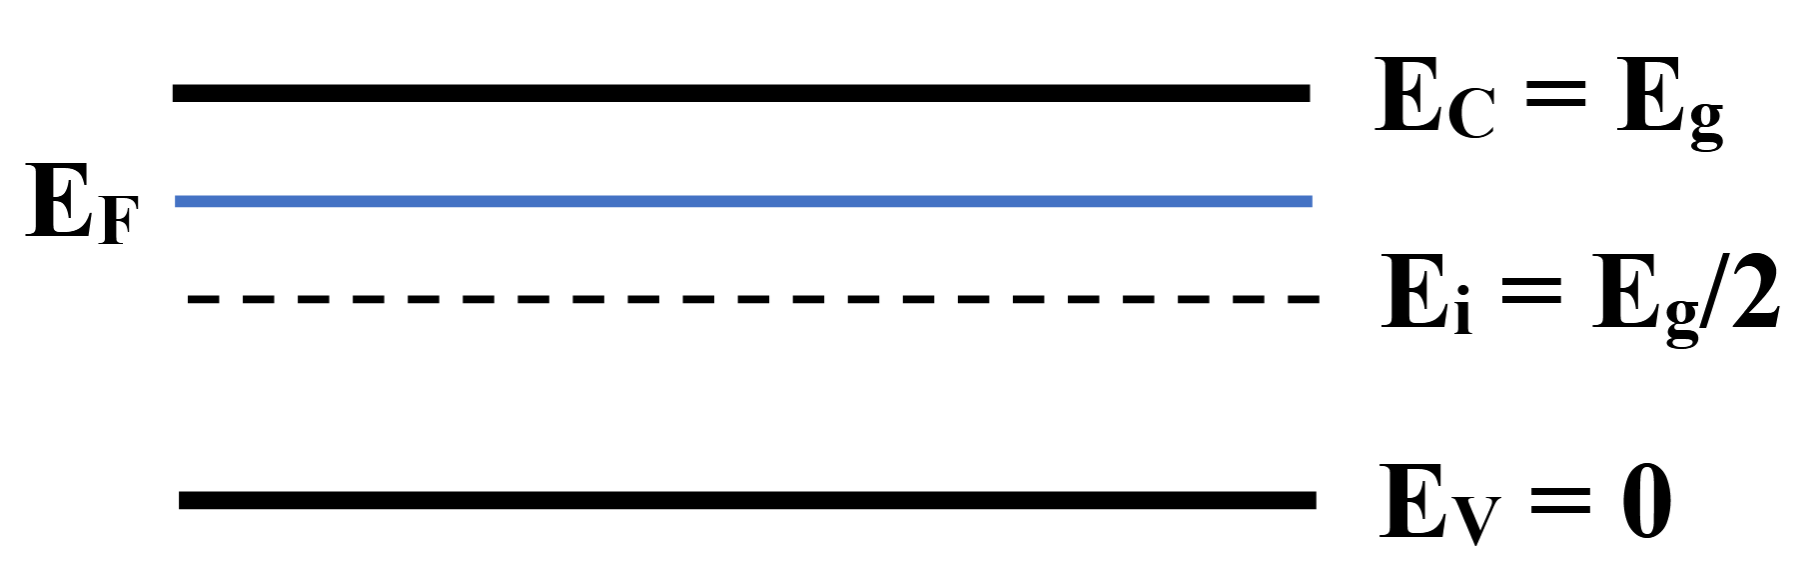
\includegraphics[width=300px]{Energies.png}
\end{figure}

\begin{table}[h]
\centering
\begin{tabular}{|P{4cm}|P{4cm}|P{4cm}|P{4cm}|}
\hline
\textbf{Material} & \textbf{Band Gap $E_{g}$ @ T = 300K(eV)} & \textbf{Effective Conduction Band Density of States $N_{C}$ @ T = 300K(cm$^{-3}$)} & \textbf{Effective Valence Band Density of States $N_{V}$ @ T = 300K(cm$^{-3}$)} \\
\hline
Silicon (Si) & 1.12 & $\num{3.22e19}$ & $\num{1.82e19}$ \\
\hline
Gallium Nitride (GaN) & 3.43 & $\num{2.3e18}$ & $\num{4.6e19}$ \\
\hline
Silicon Dioxide & 9.0 & $---$ & $---$ \\
\hline
\end{tabular}
\end{table}

\begin{enumerate}[a)]

\item An intrinsic material does not have any impurities that were intentionally introduced to increase its density of free electrons or holes. For intrinsic semiconductors (and insulators), the Fermi energy lies near the middle of the energy band gap:
$$E_{F} = E_{i} = \frac{E_{g}}{2} + \frac{k_{B}T}{2}\ln\left( \frac{N_{V}}{N_{C}} \right)$$
where $E_{i}$ is the mid-gap energy, $E_{g}$ is the energy band gap, $k_{B}$ is the Boltzmann's constant, $T$ is the temperature in Kelvin, $N_{C}$ is the effective conduction band density of states, and $N_{V}$ is the effective valence band density of states. Using the Fermi-Dirac distribution, calculate the probability that an electron is occupying the lowest-energy conduction band state at $E = E_{C} = E_{g}$ for Si, GaN, and SiO$_{2}$ at $T = 300$K. \textit{Note: }$E_{V} = 0$. 

\color{violet}
The Fermi-Dirac distribution is $f(E) = \frac{1}{1 + e^{(E - E_{F})/k_{B}T}}$. First, $E_{F}$ needs to be calculated. For silicon
\begin{gather*}
E_{F} = \frac{1.12}{2} + \frac{k_{B}T}{2}\ln\left( \frac{\num{1.82e19}}{\num{3.22e19}} \right) = 0.56 \rightarrow f(E) = \frac{1}{1 + e^{(E - E_{F})/k_{B}T}} = \num{2.939e-10}
\end{gather*}
For gallium nitride
\begin{gather*}
E_{F} = \frac{3.43}{2} + \frac{k_{B}T}{2}\ln\left( \frac{\num{4.6e19}}{2.3e18} \right) = 1.754 \rightarrow f(E) = \frac{1}{1 + e^{(E - E_{F})/k_{B}T}} = \num{6.897e-29}
\end{gather*}
For silicon dioxide
\begin{gather*}
E_{F} = \frac{9}{2} = 4.5 \rightarrow f(E) = \frac{1}{1 + e^{(E - E_{F})/k_{B}T}} = \num{2.514e-76}
\end{gather*}
\color{black}

\item For a non-degenerate semiconductor, the free electron density in the conduction band $n$ and the free hole density in the valence band $p$ are given by:
$$n = N_{C}e^{\frac{E_{F} - E_{C}}{k_{B}T}}\ \ \text{and}\ \ p = N_{V}e^{\frac{E_{V} - E_{F}}{k_{B}T}}$$
Calculate $n$ and $p$ (in cm$^{-3}$) for intrinsic Si and GaN at $T = 300$K ($E_{F} = E_{i}$ for intrinsic materials).

\color{violet}
For silicon
\begin{gather*}
n = \num{3.22e19} e^{\frac{0.56 - 1.12}{k_{B}T}} = \num{9.626e9} \\
p = \num{1.82e19} e^{\frac{-0.56}{k_{B}T}} = \num{9.463e9}
\end{gather*}
For gallium nitride
\begin{gather*}
n = \num{2.3e18}e^{\frac{1.754 - 3.43}{k_{B}T}} = \num{1.586e-10} \\
p = \num{4.6e19}e^{\frac{-1.754}{k_{B}T}} = \num{1.586e-10}
\end{gather*}
\color{black}

\item In order to increase the number of free charge carriers, impurities are intentionally added to the semiconductor in a process called \textit{doping}. Depending on the type of impurity atoms added to the semiconductor, the semiconductor can acquire additional free electrons (\textit{n-type doping}) or additional free holes (\textit{p-type doping}).

\begin{enumerate}[a)]

\item Calculate $n$ (in cm$^{-3}$) for \textit{n-type} Si and GaN at $T = 300$K when $E_{C} - E_{F} = 0.1$ eV

\color{violet}
For silicon
\begin{gather*}
n = \num{3.22e19} e^{\frac{-0.1}{k_{B}T}} = \num{6.728e17}
\end{gather*}
For gallium nitride
\begin{gather*}
n = \num{1.82e19}e^{\frac{-0.1}{k_{B}T}} = \num{3.803e17}
\end{gather*}
\color{black}

\item Calculate $p$ (in cm$^{-3}$) for \textit{p-type} Si and GaN at $T = 300$K when $E_{F} - E_{V} = 0.2$ eV. 

\color{violet}
For silicon
\begin{gather*}
p = \num{2.3e18}e^{\frac{-0.2}{k_{B}T}} = \num{1.004e15}
\end{gather*}
For gallium
\begin{gather*}
p = \num{4.6e19}e^{\frac{-0.2}{k_{B}T}} = \num{2.008e16}
\end{gather*}
\color{black}

\end{enumerate}

\end{enumerate}

\item \textbf{The Three Josephson Effects}

As discussed in lecture, a Josephson junction consists of an insulator, non-superconducting metal, or narrow region of superconducting material, known as a “weak link”, sandwiched between two superconducting regions. Cooper pairs can tunnel through the weak link region, giving rise to a current that flows across the junction. The equations that give the relationship between the junction current $I(t)$ and junction voltage $V(t)$ are:
\begin{gather*}
I(t) = I_{C}\sin(\varphi(t)) \\
\frac{\partial \varphi}{\partial t} = \frac{2eV(t)}{\hbar}
\end{gather*}
Based on the voltage applied, three separate regimes of operation are possible for a Josephson junction: the DC Josephson Effect, the AC Josephson Effect, and the Inverse AC Josephson Effect. 

\begin{enumerate}[a)]

\item \textit{DC Josephson Effect}: no voltage is applied across the junction: $V(t) = 0$.

Show that the current $I(t)$ is constant in time and non-zero in general.

\color{violet}
If $V(t) = 0$, $\frac{\partial \varphi}{\partial t} = 0$, so the change in current would be constant. Given that $\sin(\varphi(t))$ is non-zero to start, it would always be non-zero.
\color{black}

\item \textit{AC Josephson Effect}: a DC voltage is applied across the junction: $V(t) = V_{0}$.

Show that the current $I(t)$ oscillates with a frequency $\omega_{0} = 2eV_{0}/\hbar$.

\color{violet}
Given that the oscillation frequency is the rate at which the rate of change current and $V(t) = V_{0}$, $\omega_{0} = \frac{2eV_{0}}{\hbar}$. 
\color{black}

\item \textit{Inverse AC Josephson Effect}: the current through the junction consists of a DC and a microwve AC component, giving rise to a quantized DC voltage across the junction.

If the current is of form: $I(t) = I_{C}\sin(\varphi_{0} + n\omega t + \varphi_{a}\sin(\omega t))$, where $n$ is an integer, show that the DC component of the junction voltage is $V_{DC} = n\frac{\hbar}{2e}\omega$.

\color{violet}
Given that $I(t) = I_{C}\sin(\varphi(t))$, $\varphi(t)$ here must be $\varphi_{0} + n\omega t + \varphi_{a}\sin(\omega t)$. So, differentiating that would result in $\frac{\partial \varphi}{\partial t} = n\omega + \varphi_{a}\cos(\omega t)$. Given that $\frac{\partial \varphi}{\partial t} = \frac{2eV(t)}{\hbar}$, that means $V(t) = \frac{\hbar}{2e}(n\omega + \varphi_{a}\cos(\omega t))$. As time passes, that would give some $V_{DC} = \frac{\hbar n\omega}{2e}$. 
\color{black}

\end{enumerate}

\item \textbf{Quantum Algorithms}

Quantum computers show potential to perform large calculations in less time than classical computers by taking advantage of superposition and entanglement of quantum states. Just as with classical computers, quantum calculations must be implemented via an algorithm.

Choose a quantum algorithm that you find interesting and do some research to answer the following questions:

\begin{enumerate}[a)]

\item What is the name of the algorithm?

\color{violet}
The name of the algorithm is Grover's algorithm.
\color{black}

\item What problem does this algorithm solve?

\color{violet}
Grover's algorithm looks at an unsorted list and finds the index specified as an input. 
\color{black}

\item What is the practical application of this algorithm?

\color{violet}
This algorithm has uses in many classes of data retrieval and graph traversal problems, given that index finding is the very basis of all of those problems. For example, Grover's algorithm could be used to unlock cryptographic keys given enough time. 
\color{black}

\item What makes this algorithm better than its classical counterpart? If it's faster - what about it makes it faster? If there is no classical counterpart, why can't this algorithm be run on a classical computer?

\color{violet}
Grover's algorithm is able to find an answer with $O(\sqrt{N})$, whereas the classical counterpart can only manage $O(N)$. This speedup is given by the amplitude increasing capability Grover's algorithm has due to the destructive interference non-answer eigenstates are subjected to, as well as the equal probability amplitude that the initial state is in. 
\color{black}

\item Which quantum gates and/or operations are used to implement this algorithm on a quantum computer? Include a quantum circuit diagram for this algorithm if you can find one.

\color{violet}
The gates used in this algorithm include the Hadamard gate, the CNOT gate, the Pauli X gate, and the measurement gate.
\color{black}

\item Choose one of the quantum gates used by the algorithm and explain in your own words what kind of operation it performs on a qubit or qubits. 

\color{violet}
The Hadamard gate puts all the measurement qubits into superposition in the beginning of the of circuit, such that the quantum state initially is $\ket{++\dots+}$. 
\color{black}

\end{enumerate}

\end{enumerate}

\end{document}